\chapter{Appendix}
\label{ch:appendix}

\section{Code, Poster and Data}
\label{sec:app-links}

\begin{itemize}
\item Code: \url{https://github.com/Saad-Manda/PBL-Agentic-AI}. The repository has the
\texttt{trafficrl} package, the scripts and configuration files for every run, the result
CSVs in \texttt{docs/results/}, and the SHA-256 hashes of the final checkpoints in
\texttt{models/manifest.json}.
\item Poster: \posterlink
\item Data: the Jinan and Hangzhou flows of the CoLight repository \cite{wei2019colight},
\url{https://github.com/wingsweihua/colight}, commit \texttt{04440b7}. The split is defined in
\texttt{data/processed/splits.json} (\cref{sec:dataset}).
\end{itemize}

\section{Learning Curves}
\label{sec:app-curves}

\begin{figure}[ht]
\centering
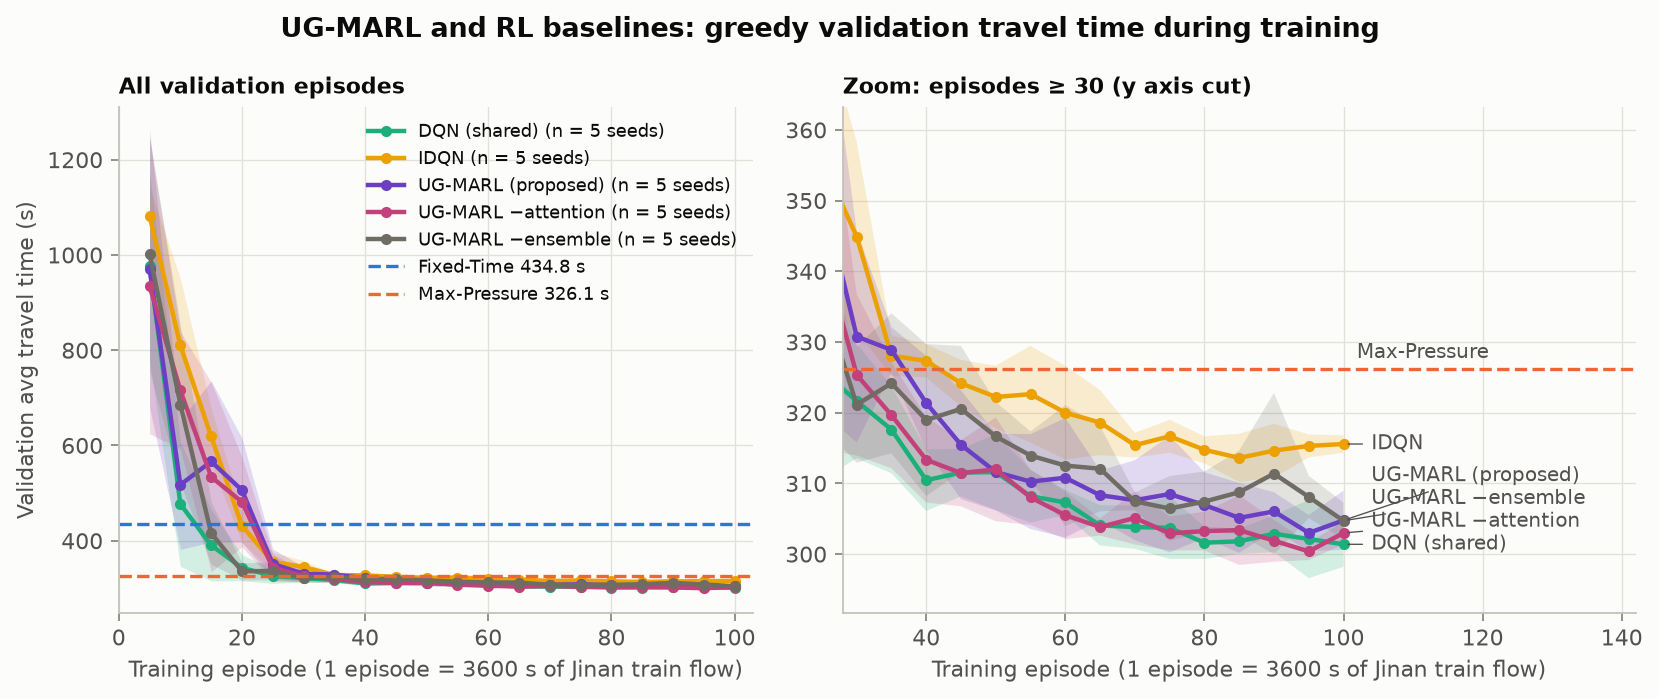
\includegraphics[width=\textwidth]{learning_curves_phase6.png}
\caption[Validation travel time during training]{Average travel time (s) of the greedy
policy on the Jinan validation flow, evaluated every 5 training episodes (mean over seeds
0--4, band = 95\,\% CI). Dashed: Fixed-Time and Max-Pressure on the same flow. Right: episodes
$\geq 30$ with the $y$ axis cut.}
\label{fig:learning-curves}
\end{figure}

Every learned controller drops below Max-Pressure between episodes 25 and 45 of its 100
training episodes (\cref{fig:learning-curves}). Over the last 30 episodes the curves move by
about as much as the seeds differ from each other, which supports the training length set in
\cref{sec:setup}. The checkpoint kept for
each seed is the evaluation with the lowest validation travel time. IDQN stays about 10\,s
above the other learners, which fits its design: each of its twelve networks learns from one
intersection's data only.
